\documentclass{AGTI} 

%% %%%%%%%%%%%%%%%%%%%%%%%%%%%%%%%%%%%%%%%%%%%%%%%%%%%%%%%%%%%%%%%%%%%%%%%%%%%%%%%%%
%% Hier bitte die Eckdaten der Arbeit eingeben (Arbeits-Typ, Titel, Name, Gutachter)
%% %%%%%%%%%%%%%%%%%%%%%%%%%%%%%%%%%%%%%%%%%%%%%%%%%%%%%%%%%%%%%%%%%%%%%%%%%%%%%%%%%

% Typ der Arbeit (z.B. Diplomarbeit, Projektarbeit, Seminararbeit,..):
%\subject{Dokumentation}
\typ{Dokumentation}

% Titel der Arbeit:
\titel{Arbeiten mit der \LaTeX-Vorlage f�r Abschlussarbeiten}

% Autor der Arbeit:
\autor{Kalle Kleinl�tzum, \\Nils Rosemann}


% Datum der Abgage (wird automatisch auf aktuelles Datum gesetzt)
\datum{\today}

% Die beiden Gutachter der Arbeit (f�r Bachelor, Master, Diplom)
\firstSupervisor{Prof. Werner Brockmann}
\secondSupervisor{Prof. Kalle Rosemann}
\erstgutachter{Prof. Werner Brockmann}
\zweitgutachter{Prof. Mr. X }

% Pfad zu den Bildern
\graphicspath{
 {./bilder/}
 {/noch/ein/verzeichnis}
}

% Eigene Makros
\newcommand{\latexklasse}{\texttt{AGTI.cls}}

  
\begin{document}

% F�r eine sch�nere Ausgabe f�r zu Hause oder f�r den Betreuer besteht
% hier die M�glichkeit, der Arbeit mit einem zus�tzlichen schmucken Deckblatt 
% (mit Titelbild) eine pers�nliche Note zu verleihen: 
% Dazu dem Befehl \extraTitelblatt einen \includegraphics-Befehl �bergeben
%\extraTitelblatt{\fbox{
\includegraphics[width=.52\linewidth]{titelbild}}}
%\cleardoublepage

% Dieser Befehl erzeugt das offizielle Titelblatt
\standardTitelblatt
\cleardoublepage

% Dieser "normale" Titel-Erzeugungsbefehl wird nicht mehr ben�tigt
%\maketitle
%\newpage 
%\cleardoublepage

% Durch den folgenden Befehl wird die Erkl�rung eingebunden,
% dass man die Arbeit seri�s erstellt hat.

% \erklaerung%%{\today}
% \cleardoublepage

% Hier die Zusammenfassung auf Deutsch und auf Englisch
\thispagestyle{empty}
\section*{Zusammenfassung}
Bei allen Abschlussarbeiten wird zu Beginn der Arbeit eine kurze Zusammenfassung in deutscher und englischer Sprache verlangt. Diese d�rfen zusammen maximal eine Seite einnehmen.
\vfill
\section*{Abstract}
In the preface of all thesis, a short abstract of the work is required both in german and in english language. The length for both is restricted to one page maximum.
\cleardoublepage

% Hier kommt bei umfangreichen Arbeiten (Master- oder Diplomarbeit) ein Vorwort
%   \chapter*{Vorwort}
%   Da bei Master-- und Diplomarbeiten im Allgemeinen ein Vorwort erwartet
%   wird, soll beispielhaft auch bei dieser Dokumentation ein solches
%   erscheinen.  Bei Arbeiten geringeren Umfanges ist ein Vorwort
%   nicht unbedingt angebracht.
%   
%   Zumeist finden sich in Vorworten irgendwelche Danksagungen. Wem man
%   dankt, sei jedem selber �berlassen, wir m�chten an dieser Stelle 
%   Roland Bless, Tobias Luksch, Kai Lingemann und Andreas N�chter
%   danken, auf deren Vorarbeiten dieses Dokument sowie die zugeh�rige 
%   \LaTeX-Klasse basieren.
% \cleardoublepage

\pagenumbering{roman}
\tableofcontents

\cleardoublepage

%%%%%%%%%%%%%%%%%%%%%%%%%%%%%%%%%%%%%%%%%%%%%%%%%%%%%%%%%%%%
%% Beginn der eigentlichen Arbeit
%%
%% Bei l�ngeren Arbeiten ist es sinnvoll, Kapitel in 
%% einzelne Dateien auszulagern, die dann in der Hauptdatei
%% mittels \include{} eingebunden werden
%%%%%%%%%%%%%%%%%%%%%%%%%%%%%%%%%%%%%%%%%%%%%%%%%%%%%%%%%%%%

% Seitennummer auf 1 setzen

\pagenumbering{arabic}

%%%%%%%%%%%%%%%%%%%%%%%%%%%%%%%%%%%%%%%%%%%%%%%%%%%%%%%%%%%%
%% einleitung.tex
%%
%% Kapitel: Einleitung
%% Hauptdokument: howto.tex
%% Autor: Tobias Luksch
%% Datum: Juli 2003
%%%%%%%%%%%%%%%%%%%%%%%%%%%%%%%%%%%%%%%%%%%%%%%%%%%%%%%%%%%%
\chapter{Einleitung}
\label{chap:einl}

%%%%%%%%%%%%%%%%%%%%%%%%%%%%%%%%%%%%%%%%%%%%%%%%%%%%%%%%%%%%
\section{Motivation}
\label{sec:einl:motiv}
%%%%%%%%%%%%%%%%%%%%%%%%%%%%%%%%%%%%%%%%%%%%%%%%%%%%%%%%%%%%
Die Arbeitsgruppe Technische Informatik an der
Universit�t Osnabr�ck bietet eine Vielzahl von Angeboten an
studentischen Arbeiten an, seien es Abschlussarbeiten,
Seminare oder Praktika. F�r all diese Arbeiten ist ein Dokument zu
erstellen, das die Anspr�che an eine wissenschaftliche Arbeit erf�llen
sollte. Um es den Studierenden einfacher zu machen, diesen Anspr�chen
gerecht zu werden, bietet die Arbeitsgruppe \LaTeX -Vorlagen an,
die ein professionelles und einheitliches Layout erm�glichen.
% Diese Dokumentation 
% beschreibt die Formatvorlage f�r \emph{Abschlussarbeiten}.

%%%%%%%%%%%%%%%%%%%%%%%%%%%%%%%%%%%%%%%%%%%%%%%%%%%%%%%%%%%%
\section{Ziel der Arbeit}
\label{sec:einl:ziel}
%%%%%%%%%%%%%%%%%%%%%%%%%%%%%%%%%%%%%%%%%%%%%%%%%%%%%%%%%%%%
Das Ziel dieser Dokumentation ist es, Studierenden eine Anleitung zum
Erstellen wissenschatlicher Dokumente an die Hand zu geben. Dabei wird
auf Besonderheiten der zur Verf�gung gestellen \LaTeX -Klasse ebenso
eingegangen wie auf einige prinzipelle Formalismen wissenschatlicher
Arbeiten. Es wird aufgezeigt, wie Bilder oder Tabellen korrekt
erstellt und referenziert werden und wie ein Literaturverzeichnis
erstellt wird. Dieses Dokument selbst dient als Beispiel und kann als
Vorlage und Ausgangspunkt f�r eigene Arbeiten verwendet werden.

Es sei angemerkt, dass dies weder eine Einf�hrung in \LaTeX\ ist, noch wird
eine Anleitung zur Installation von \LaTeX -Distributionen gegeben.
Dazu sei deshalb auf die einschl�gige Literatur (zum Beispiel
\cite{Lamport95}, \cite{Goossens96}) oder Webseiten (\cite{WWWDante},
\cite{WWWMikTex}) verwiesen.

Weiterhin sei bemerkt, dass der Sprachstil dieser Arbeit �ber weite
Teile (nicht �berall) formaler gehalten ist als notwendig.
Der Grund hierf�r liegt in der Intention, dem Leser einen Eindruck zu
vermitteln, welcher Art der Stil einer wissenschaftlichen Arbeit sein
sollte. Man m�ge dem Autor deshalb den Mangel an Lockerheit und
humoristischen Ausschweifungen verzeihen.

% %%%%%%%%%%%%%%%%%%%%%%%%%%%%%%%%%%%%%%%%%%%%%%%%%%%%%%%%%%%%
% \section{Aufbau der Arbeit}
% \label{sec:einl:aufbau}
% Kapitel~\ref{chap:klasse} besch�ftigt sich zun�chst mit der von der AG
% Robotersysteme angebotenen \LaTeX -Klasse \latexklasse. Es wird
% erl�utert, welche Form das Hauptdokument haben muss und welche Makros
% zur Verf�gung gestellt werden.
% 
% Anschlie�end finden sich in Kapitel~\ref{chap:floats} Anleitungen zum
% Erstellen besonderer Dokumentelemente. Bilder und Tabellen werden
% ebenso behandelt wie Formeln oder Literaturverweise.
% 
% In Kapitel~\ref{chap:aufbau} werden einige kurze Hinweise zum
% allgemeinen Aufbau einer wissenschaftlichen Arbeit gegeben. Dies ist
% nur als Anregung zu verstehen, eine ausgiebige Einf�hrung hierzu w�rde
% den Rahmen dieser Dokumentation sprengen.


%%% Local Variables: 
%%% mode: latex
%%% TeX-master: "howto"
%%% End: 


%%%%%%%%%%%%%%%%%%%%%%%%%%%%%%%%%%%%%%%%%%%%%%%%%%%%%%%%%%%%
%% latexklasse.tex
%%
%% Kapitel: Die Latex-Klasse agrosy.cls
%% Hauptdokument: howto.tex
%% Autor: Tobias Luksch
%% Datum: Juli 2003
%%%%%%%%%%%%%%%%%%%%%%%%%%%%%%%%%%%%%%%%%%%%%%%%%%%%%%%%%%%%
\chapter{Aufbau der \LaTeX -Vorlage}
\label{chap:aufbau}
Dieses Kapitel behandelt die zur Verf�gung gestellte \LaTeX -Klasse
\latexklasse\ und die aus ihrer Anwendung resultierende Struktur des
Hauptdokumentes. Die wichtigsten Makros werden erl�utert und ein paar
Hinweise zum systematischen Aufbau der Arbeit gegeben.

%%%%%%%%%%%%%%%%%%%%%%%%%%%%%%%%%%%%%%%%%%%%%%%%%%%%%%%%%%%%
\section{Grundfunktionen des Hauptdokumentes}
\label{sec:aufbau:hauptdoku}
%%%%%%%%%%%%%%%%%%%%%%%%%%%%%%%%%%%%%%%%%%%%%%%%%%%%%%%%%%%%
\index{Hauptdokument}\index{\latexklasse} Das Hauptdokument (englisch
\emph{master file}), h�lt sich an die �bliche Form eines \LaTeX
-Dokumentes. Grunds�tzlich kann das Hauptdokument dieser Dokumentation
(\texttt{howto.tex}) als kommentiertes Beispiel herangezogen werden.
Als Klasse ist im Kopf des Dokumentes (\verb|\documentclass{}|)
\latexklasse\ anzugeben.
Es folgen die �blichen Angaben zu Titel, Autor und Typ der Arbeit, im
einzelnen \verb|\titel|, \verb|\autor|, \verb|\typ| (Bachelorarbeit,
Diplomarbeit,\dots) und Felder f�r die Gutachter, die bei Abschlussarbeiten
angegeben werden sollten. Dann bietet sich noch die M�glichkeit,
eigene Makros zu definieren und \index{Bilder!Verzeichnisse}
Verzeichnisse anzugeben, in denen nach Bildern gesucht werden soll
(\verb|\graphicspath|).
Anschlie�end beginnt der sichtbare Inhalt innerhalb der
\verb|document|-Umbegung. Hier k�nnen bestimmte Makros verwendet werden:
\begin{description}
\item[$\backslash$maketitle] generiert die Titelseite mit Titel und
  Autor der Arbeit
\item[$\backslash$erklaerung] erstellt eine Seite, die aussagt, dass
  der Autor die Arbeit selbst�ndig verfasst und alle benutzten Quellen
  angegeben hat. Diese Seite ist bei offiziellen Exemplaren vom Autoren zu 
  unterschreiben.
% \item[$\backslash$prefacesection] bietet die M�glichkeit, Zusammenfassung
%   und Abstract einzuf�gen. Auch Danksagungen lassen sich damit erstellen.
%   Als Beispiel sei auf die Quellen dieses Textes
%   verwiesen.
\item[$\backslash$tableofcontents] f�gt das Inhaltsverzeichnis ein.
\item[$\backslash$bibliography] erzeugt das Literaturverzeichnis. Als
  Parameter wird die zu verwendende BibTex-Datei (ohne \verb|.bib|)
  �bergeben. Mehr zu Literaturhinweisen in
  Kapitel~\ref{sec:floats:bib}.
\end{description}
%
Bei l�ngeren Arbeiten kann es sinnvoll sein, auch einen Index zu erstellen.
Dazu sei auf die einschl�gige \LaTeX-Literatur verwiesen.
Tabelle~\ref{tab:dateien} gibt eine �bersicht der zur \LaTeX -Vorlage geh�renden Dateien.
%
\begin{table}
  \centering
  \caption{Die bereitgestellten Dateien mit einer kurzen Beschreibung.} \vskip 2mm
  \begin{tabular}[c]{lp{10cm}}
    \hline
    \bf Dateiname & \bf Beschreibung \\
    \hline 
    \latexklasse & Die Klassendefinition beruhend auf scrreprt.cls \\
    \texttt{howto.tex} & Die Hauptdatei dieser Dokumentation \\
    \texttt{kapitel/} & Das Verzeichnis, in dem die Kapitel (in \texttt{tex}-Files) liegen\\
    \texttt{literatur.bib} & Die Literaturliste zu diesem Dokument im BibTeX-Format \\
    \texttt{beispiele.bib} & Kommentierte Beispieldatei zur BibTex-Datenbank \\
    \texttt{algorithmen/} & Verzeichnis mit Style-Dateien und Dokumentation zum Einbau von Algorithmen \\
%     \texttt{algorithms.ps, .tex} & Dokumentation zu den Algorithmus-Styles \\
%    \texttt{makefile} & Makefile zur automatischen Generation des Dokuments \\
    \hline
  \end{tabular}
%  \caption{Die bereitgestellten Dateien mit einer kurzen Beschreibung.}
  \label{tab:dateien}
\end{table}


%%%%%%%%%%%%%%%%%%%%%%%%%%%%%%%%%%%%%%%%%%%%%%%%%%%%%%%%%%%%
\section{Hilfreiche Tipps}
\label{sec:aufbau:tipps}
%%%%%%%%%%%%%%%%%%%%%%%%%%%%%%%%%%%%%%%%%%%%%%%%%%%%%%%%%%%%
In diesem Abschnitt werden einige Tipps zur Strukturierung und Handhabung
der Arbeit gegeben.

%%%%%%%%%%%%%%%%%%%%%%%%%%%%%%%%%%%%%%%%%%%%%%%%%%%%%%%%%%%%
\subsection{Kapitel in externen Dateien}
\label{sec:aufbau:tipps:kapitel}
%%%%%%%%%%%%%%%%%%%%%%%%%%%%%%%%%%%%%%%%%%%%%%%%%%%%%%%%%%%%
\index{Kapitel}
Bei l�ngeren Dokumenten ist es grunds�tzlich ratsam, den Text
auf mehrere Dateien zu verteilen, zum Beispiel f�r
jedes Kapitel eine eigene Datei anzulegen. Diese k�nnen dann mittels
des \verb|\include|-Befehls in der Hauptdatei eingef�gt werden. Auch
diese Dokumentation ist derart gegliedert, die einzelnen Kapitel befinden 
sich im Verzeichnis \texttt{kapitel}.

%%%%%%%%%%%%%%%%%%%%%%%%%%%%%%%%%%%%%%%%%%%%%%%%%%%%%%%%%%%%
\subsection{Label}
\label{sec:aufbau:tipps:label}
%%%%%%%%%%%%%%%%%%%%%%%%%%%%%%%%%%%%%%%%%%%%%%%%%%%%%%%%%%%%
\index{Label}
Ein Hilfsmittel, von dem man unbedingt Gebrauch machen sollte, ist die Verwendung von {\it Labeln}. Diese funktionieren so, dass jeder Abschnitt und jedes Bild mit einem eindeutigen Label versehen wird, welches zum Verweis auf den betreffenden Abschnitt bzw. das Bild verwendet wird. Dank dieser Label bleibt die Referenzierung von Dokumenteninhalten auch bei Umstellung von Abschnitten und Kapiteln immer konsistent. So kann von diesem Dokument z.B. immer guten Gewissens behauptet werden, dass Abbildung~\ref{fig:bisam} auf Seite~\pageref{fig:bisam} steht und Abschnitt~\ref{sec:aufbau:tipps:label} auf Seite~\pageref{sec:aufbau:tipps:label} beginnt.\\
Bei der Wahl der Label bietet es sich an, eine
einheitliche Benennung zu w�hlen. Diese Dokumentation benennt Label
nach dem Schema \verb|<type>:<beschreibung>|, wobei \verb|<type>| zum
Beispiel \verb|chap|, \verb|sec|, \verb|fig|, \verb|eq| oder etwas
entsprechendes sein kann. Das mag zwar alles etwas mehr Tipperei sein,
verbessert jedoch die Lesbarkeit des Dokumentes erheblich und spart 
zus�tzlich viel Arbeit.

%%%%%%%%%%%%%%%%%%%%%%%%%%%%%%%%%%%%%%%%%%%%%%%%%%%%%%%%%%%%
\subsection{Kommentare}
\label{sec:aufbau:tipps:kommentare}
%%%%%%%%%%%%%%%%%%%%%%%%%%%%%%%%%%%%%%%%%%%%%%%%%%%%%%%%%%%%
\index{Kommentare}
In \LaTeX\ sind Kommentare erlaubt (beginnend mit \verb|%|), also
sollte man davon Gebrauch machen. Hilfreich sind deutliche Einschnitte
zwischen Unterkapiteln oder anderen relevanten Abschnitten, so dass
man sich schneller in seinen Quellen zurechtfindet.

Verwendet man unter Linux (X-)Emacs zum Schreiben der Arbeit, 
l�sst sich in den Unterdateien durch einen Block der Art
\begin{verbatim}
   %%% Local Variables: 
   %%% mode: latex
   %%% TeX-master: "howto"
   %%% End: 
\end{verbatim}
am Ende der Datei auf die Hauptdatei verweisen. Das Programm weiss
dadurch, welche Datei zu kompilieren bzw. anzuzeigen ist. Verwendet
man unter Windows das Programm TeXnicCenter l�sst sich eine �hnliche
Funktionalit�t mittels Projekten erreichen.

%%%%%%%%%%%%%%%%%%%%%%%%%%%%%%%%%%%%%%%%%%%%%%%%%%%%%%%%%%%%
\subsection{Kompilieren des Dokumentes}
\label{sec:aufbau:tipps:kompilieren}
%%%%%%%%%%%%%%%%%%%%%%%%%%%%%%%%%%%%%%%%%%%%%%%%%%%%%%%%%%%%
\index{Kompilieren}
Kurz ein paar Worte zum Kompilieren der \LaTeX -Quellen. Unter Windows
und dem TeXnicCenter sollte das gr��tenteils automatisch passieren.
Unter Linux kann es sein, dass man mehrfach kompilieren muss, um die
Referenzen richtig zu kriegen. Ein komplettes Kompilieren sieht zum
Beispiel so aus:
\begin{verbatim}
   > latex howTo.tex
   > makeindex howTo.idx
   > bibtex howTo.aux
   > latex howTo.tex
   > latex howTo.tex
   >
\end{verbatim} 
Diese Schritte lassen sich aber auch durch ein \emph{makefile}, ein
\emph{SConscript} oder Shellskripte automatisieren.

%%% Local Variables: 
%%% mode: latex
%%% TeX-master: "howto"
%%% End: 


%%%%%%%%%%%%%%%%%%%%%%%%%%%%%%%%%%%%%%%%%%%%%%%%%%%%%%%%%%%%
%% floats.tex
%%
%% Kapitel: Tabellen, Bilder und mehr
%% Hauptdokument: howto.tex
%% Autor: Tobias Luksch
%% Datum: Juli 2003
%%%%%%%%%%%%%%%%%%%%%%%%%%%%%%%%%%%%%%%%%%%%%%%%%%%%%%%%%%%%
\chapter{Tabellen, Bilder und mehr}
\label{chap:floats}
%%%%%%%%%%%%%%%%%%%%%%%%%%%%%%%%%%%%%%%%%%%%%%%%%%%%%%%%%%%%
Damit auch Bilder, Tabellen etc. und deren Beschriftung und
Referenzierung einheitlich erscheinen, beschreibt dieses Kapitel, wie
eben diese Elemente eingebunden werden sollten.

%%%%%%%%%%%%%%%%%%%%%%%%%%%%%%%%%%%%%%%%%%%%%%%%%%%%%%%%%%%%
\section{Bilder}
\label{sec:floats:bilder}
\index{Bilder} 
%%%%%%%%%%%%%%%%%%%%%%%%%%%%%%%%%%%%%%%%%%%%%%%%%%%%%%%%%%%%
In ein \LaTeX-Dokument k�nnen Bilder verschiedener Formate eingef�gt werden, 
jedoch abh�ngig vom gew�nschten Zielformat: Wird {\it normales} \texttt{latex}
 mit dem Zielformat postscript benutzt, k�nnen nur Bilder im \texttt{PS}- und 
im \texttt{EPS}-Format eingebunden werden. Wird \texttt{pdflatex} zum direkten 
Erzeugen von pdf-Dateien verwendet, k�nnen keine \texttt{PS}- und \texttt{EPS}-Bilder 
verwendet werden, daf�r \texttt{PDF}s, \texttt{JPG}s und \texttt{PNG}s.  
Um den Studierenden die Wahl des Zielformats zu erm�glichen, 
ist folgende Konvention n�tig: 
\begin{quote}
Jedes eingebundene Bild wird doppelt gespeichert: Einmal in \texttt{PS}- oder \texttt{EPS}-Format und einmal in \texttt{PDF}-, \texttt{JPG}- oder \texttt{PNG}-Format.
Beim Einbinden in das \TeX-Dokument wird dann der Dateiname ohne Endung angegeben. \texttt{Latex} bzw. \texttt{pdflatex} suchen sich dann automatisch die richtige Datei.
\end{quote}
Unter Linux k�nnen die Bilder mit Kommandos wie \verb|epstopdf| und \verb|pdf2ps| sowie mit Grafikprogrammen wie Gimp ineinander �berf�hrt werden, unter Windows empfiehlt sich auf jeden Fall Gimp oder ein entsprechendes Grafikprogramm. Unabh�ngig von dem Format, in dem die Bilder gespeichert werden, sollte auf eine ausreichend hohe Aufl�sung geachtet werden, damit die Bilder nicht pixelig erscheinen.

\begin{figure}
  \begin{center}
    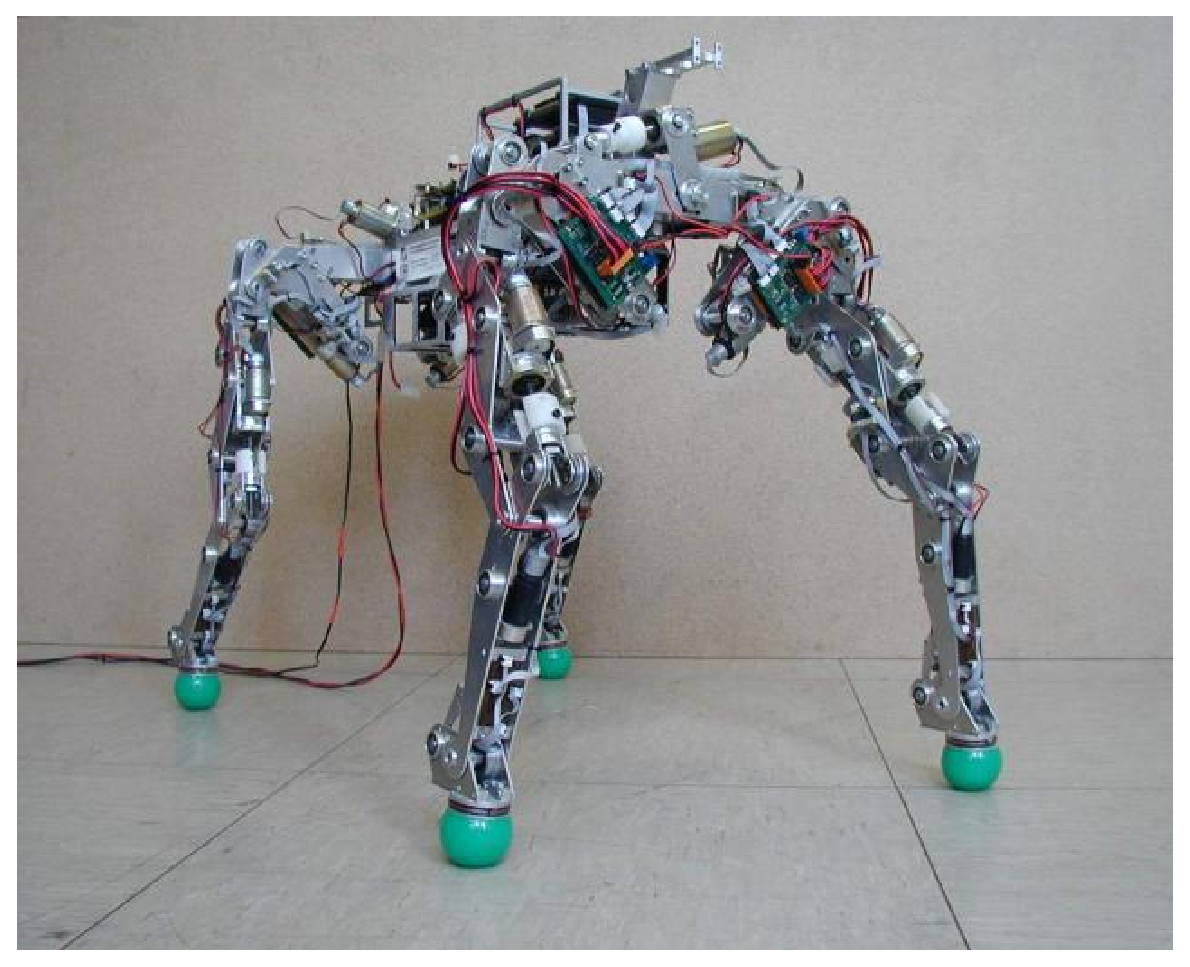
\includegraphics[width=10cm]{bisam}
    \caption{Die vierbeinige Laufmaschine \textsc{Bisam}, 
      die am Forschungszentrum Informatik in Karlsruhe entwickelt
      wurde.}
    \label{fig:bisam}
  \end{center}
\end{figure}

Um Bilder einzuf�gen verwendet man eine \texttt{figure}-Umgebung wie:
\begin{verbatim}
   \begin{figure}
     \begin{center}
       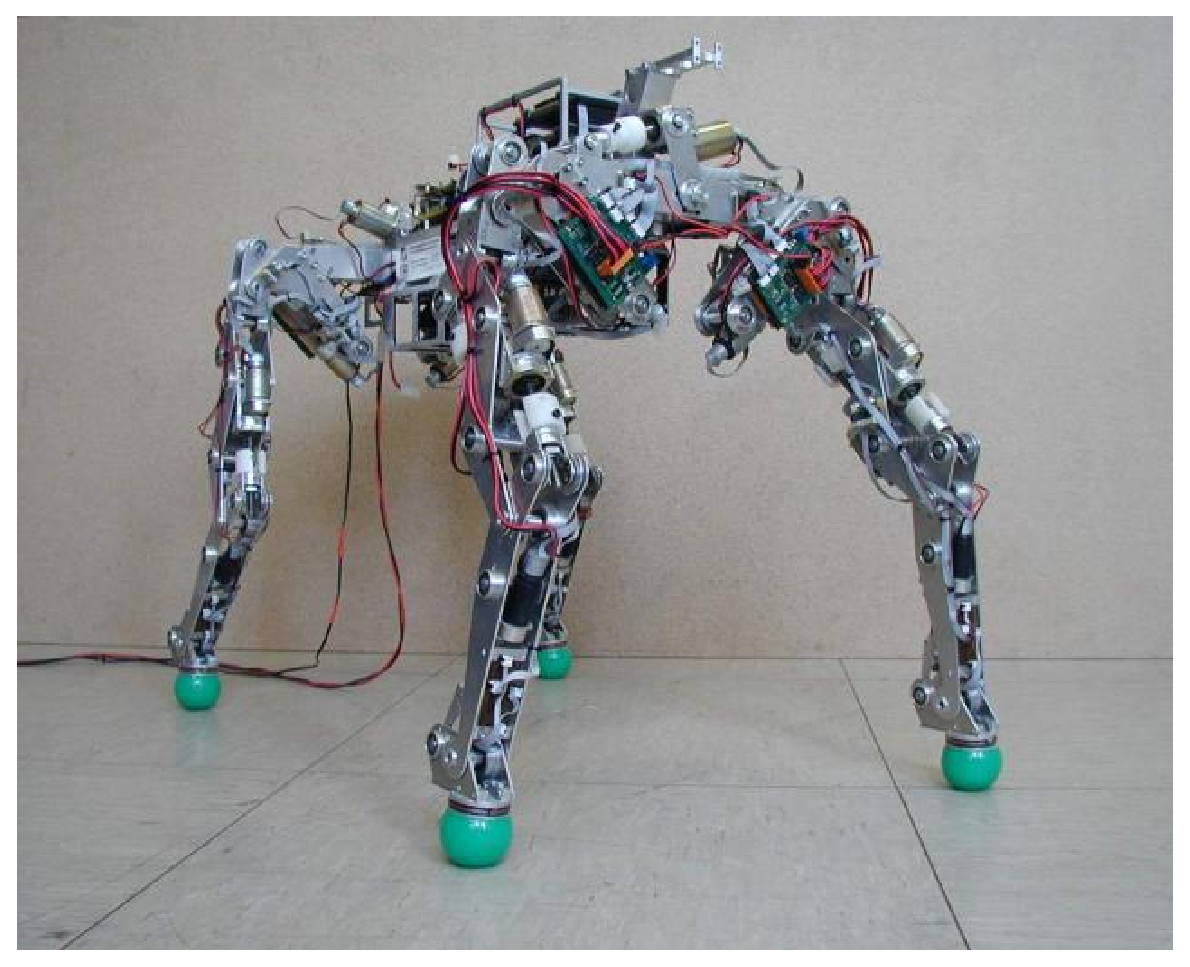
\includegraphics[width=10cm]{bisam}
       \caption{Die vierbeinige Laufmaschine \textsc{Bisam}, 
         die am Forschungszentrum Informatik in Karlsruhe entwickelt
         wurde.}
       \label{fig:bisam}
     \end{center}
   \end{figure}
\end{verbatim}
Dies erzeugt die Ausgabe, die in Abbildung~\ref{fig:bisam} zu sehen
ist. Zu den einzelnen Befehlen und ihren Parametern sei auf
entsprechende Literatur verwiesen. 

Wichtig ist, dass die
Bildunterschrift auch wirklich beschreibt, was mit dem Bild gezeigt
werden soll. Die Diskussion des Gezeigten sollte sich allerdings im
Flie�text befinden. Ist die Abbildung z.B. ein Plot, k�nnte die
Beschriftung hei�en: ``Der Temperaturverlauf bei geschlossenem Ventil
B. Hier �berschreitet die Temperatur die kritische Grenze bei
$t=130\mbox{sec}$''. Warum das aber so ist, welche Effekte eine Rolle
spielen oder ob das gut oder schlecht ist, geh�rt nicht unter das
Bild, sondern sollte im Text diskutiert werden. Bei Datenplots ist
�brigens grunds�tzlich darauf zu achten, dass alle Achsen sauber
beschriftet sind und die Legende vollst�ndig ist. Bei zusammengeh�rigen
Bildern ist zus�tzlich auf eine einheitliche Skalierung und Beschriftung 
zu achten.

%%%%%%%%%%%%%%%%%%%%%%%%%%%%%%%%%%%%%%%%%%%%%%%%%%%%%%%%%%%%
\section{Tabellen}
\label{sec:floats:tabellen}
%%%%%%%%%%%%%%%%%%%%%%%%%%%%%%%%%%%%%%%%%%%%%%%%%%%%%%%%%%%%
\index{Tabellen} F�r die Beschriftung von Tabellen gilt im Prinzip das
bei Bildern Gesagte. Mit der Anzahl der Linien kann man etwas
herumexperimentieren, allerdings sollte das Aussehen der Tabellen in
der ganzen Arbeit konsistent sein. Tabelle~\ref{tab:dateien} kann als
Beispiel f�r Tabellen herangezogen werden.

%%%%%%%%%%%%%%%%%%%%%%%%%%%%%%%%%%%%%%%%%%%%%%%%%%%%%%%%%%%%
\section{Formeln}
\label{sec:floats:formeln}
%%%%%%%%%%%%%%%%%%%%%%%%%%%%%%%%%%%%%%%%%%%%%%%%%%%%%%%%%%%%
\index{Formeln} Formeln sollten nicht im Flie�text untergehen, auch
wenn es nur kleine (und einfallslose) sind wie $E=mc^2$, sondern
vielmehr in einer \verb|equation|-Umgebung ausgegeben werden:
\begin{equation}
  \label{eq:einstein}
  E=mc^2 
\end{equation}
Grunds�tzlich sollten Formeln nummeriert werden, bei l�ngeren
Herleitungen reicht es jedoch, nur wichtige Schritte und das
Endergebnis zu benennen. Werden im Flie�text Variablen genannt, wie
zum Beispiel die Energie $E$ oder die Lichtgeschwindigkeit $c$ aus
Gleichung~\ref{eq:einstein}, so sollten diese im Mathematikmodus
gesetzt sein (z.B. \verb|$E$|).

%%%%%%%%%%%%%%%%%%%%%%%%%%%%%%%%%%%%%%%%%%%%%%%%%%%%%%%%%%%%
\section{Algorithmen}
\label{sec:floats:algo}
%%%%%%%%%%%%%%%%%%%%%%%%%%%%%%%%%%%%%%%%%%%%%%%%%%%%%%%%%%%%
\index{Algorithmen} Zum Visualisieren von Algorithmen und besonderen
Programmabschnitten kann die Funktionalit�t der Pakete
\verb|algorithm.sty| und \verb|algorithmic.sty| verwendet werden.
Beide werden zum Beispiel auf \cite{WWWDante} als unterst�tzt gef�hrt,
sind allerdings im Allgemeinen nicht bei \LaTeX -Distributionen dabei,
weshalb wir sie mitliefern.

\begin{algorithm}
\begin{algorithmic}[5]  %% opt. Param.: alle n Zeilen Zeilennummer
\STATE Lege 2D-Array an
\STATE{F�hre Tiefensuche durch:}
\FORALL{Knoten des Baumes $U$ mit Koordinaten $(x,y,z)$}
  \IF{$z$-Koordinate der Zelle gr��er als in Wert im Array an $(x,y)$}
    \STATE Speichere $z$ an der Stelle $(x,y)$ in 2D-Array
  \ENDIF
\ENDFOR
\STATE Lege Quadtree $G$ an
\STATE{F�hre erneut Tiefensuche durch:}
\FORALL{Knoten des Baumes $U$ mit Koordinaten $(x,y,z)$}
  \IF{Koordinaten identisch mit den im 2D-Array gespeicherten}
    \STATE{Speichere $z$ f�r $(x,y)$ im Quadtree $G$}
  \ENDIF
\ENDFOR
\end{algorithmic}
\caption{Generieren einer globalen 2D-Karte $G$ aus Urkarte $U$}
\label{alg:beispiel}
\end{algorithm}

Als Dokumentation ist die Datei \verb|algorithms.ps| einschlie�lich
ihrer \LaTeX -Quellen \verb|algorithms.tex| beigef�gt. Grunds�tzlich
sollten wichtige Algorithmen als Pseudocode in der Art von
Algorithmus~\ref{alg:beispiel} mithilfe dieser Pakete angegeben
werden, um das Verst�ndnis zu erleichtern. Sollte es tats�chlich n�tig
sein, ``richtigen'' Quellcode einzuf�gen (der aber h�chstens mal in
den Anhang geh�rt), ist der \LaTeX -Style \verb|listings.sty|
empfehlenswert.


%%%%%%%%%%%%%%%%%%%%%%%%%%%%%%%%%%%%%%%%%%%%%%%%%%%%%%%%%%%%
\section{Literaturverweise}
\label{sec:floats:bib}
%%%%%%%%%%%%%%%%%%%%%%%%%%%%%%%%%%%%%%%%%%%%%%%%%%%%%%%%%%%%
\index{Literaturverweise} Nat�rlich m�ssen s�mtliche verwendete
Quellen aufgef�hrt werden. Dazu sind sie im Literaturverzeichnis zu
verzeichnen und an der entsprechenden Textstelle ist auf sie zu
verweisen. Letzteres geschieht mit \verb|\cite{<label>}|, wobei
\verb|<label>| der zugeh�rige Eintrag in der BibTex-Datei ist. Der
Name der BibTex-Datei wird im Hauptdokument dem \verb|literatur|-Makro
�bergeben (siehe auch Abschnitt~\ref{sec:aufbau:hauptdoku}). Zum Aufbau der
BibTex-Datei kann ein Blick in \verb|literatur.bib| geworfen
oder entsprechende Literatur (\cite{Lamport95}, \cite{WWWBibTex})
konsultiert werden. Au�erdem finden sich in der Datei
\verb|beispiele.bib| exemplarische BibTex-Eintr�ge der meisten verwendeten 
Literaturquellen mit einer kurzen Erkl�rung.

Das verwendete BibTex-Layout erzeugt Verweise bestehend aus dem
Nachnamen des ersten Autors und den letzten beiden Ziffern der
Jahreszahl. Bei Verweisen auf URLs sollte der \verb|@Misc|-Eintrag
derart verwendet werden, wie es in \verb|literatur.bib| zu finden ist.

--> Siehe z.B. \cite{Albiez03}.

Auf URL-Verweise sollte jedoch so weit wie m�glich verzichtet werden,
da Printmedien wie Paper, B�cher und wissenschaftliche Artikel diesen
grunds�tzlich vorzuziehen sind. D.h., zu Ver�ffentlichungen, die per
Internetsuche gefunden wurden, sollten so weit wie m�glich auch
zitierf�hige Angaben gesucht werden. Die Aktualit�t von URLs sollte
auch immer durch ein Datum (Monat und Jahr) angezeigt werden.

%%%%%%%%%%%%%%%%%%%%%%%%%%%%%%%%%%%%%%%%%%%%%%%%%%%%%%%%%%%%
\section{Index}
\label{sec:floats:index}
%%%%%%%%%%%%%%%%%%%%%%%%%%%%%%%%%%%%%%%%%%%%%%%%%%%%%%%%%%%%
\index{Indexverzeichnis} 
In gr��eren Arbeiten kann es sinnvoll sein, einen Index zu erstellen, ein Abbildungsverzeichnis ist dagegen meistens �berfl�ssig. 
Das Indexverzeichnis erstellt man am besten, wenn man mit der
Ausarbeitung fertig ist, indem man die Arbeit noch einmal Abschnitt f�r Abschnitt 
durchgeht und bei jedem (inhaltlich neuen) Abschnitt das behandelte Thema (oder mehrere) ``auf den Index'' setzt. Dies geschieht mit dem Indexverweis: \\
\verb|   \index{<Stichwort>}|, \\
wodurch dieses <Stichwort> dann im Indexverzeichnis zusammen mit der
Seitenzahl, auf der der \verb|index|-Befehl steht, aufgef�hrt wird.
Unterpunkte lassen sich mit \\
\verb|   \index{<Stichwort>!<Unterpunkt>}| \\
erzeugen. Das Indexverzeichnis selbst wird im Masterdokument zentral mit dem
Makro \verb|\indexverzeichnis| generiert.



%%% Local Variables: 
%%% mode: latex
%%% TeX-master: "howto"
%%% End: 


%%%%%%%%%%%%%%%%%%%%%%%%%%%%%%%%%%%%%%%%%%%%%%%%%%%%%%%%%%%%
%% inhalt.tex
%%
%% Kapitel: Inhaltliche Gestaltung,
%% Kapitel: Bewertungsrichtlinien
%% Hauptdokument: howto.tex
%% Autor: Kalle Kleinl�tzum
%% Datum: August 2007
%%%%%%%%%%%%%%%%%%%%%%%%%%%%%%%%%%%%%%%%%%%%%%%%%%%%%%%%%%%%
\chapter{Inhaltliche Gestaltung}
\label{chap:inhalt} \index{Inhalt}
%%%%%%%%%%%%%%%%%%%%%%%%%%%%%%%%%%%%%%%%%%%%%%%%%%%%%%%%%%%%
Dieses Kapitel befasst sich n�her mit dem Inhalt einer Abschlussarbeit. Es 
beschreibt den �blichen Aufbau und gibt Hinweise zu h�ufig gemachten 
Fehlern sowie zum Sprachgebrauch.

%%%%%%%%%%%%%%%%%%%%%%%%%%%%%%%%%%%%%%%%%%%%%%%%%%%%%%%%%%%%
\section{Aufbau einer Abschlussarbeit}
\label{sec:inhalt:aufbau} \index{Aufbau} 
%%%%%%%%%%%%%%%%%%%%%%%%%%%%%%%%%%%%%%%%%%%%%%%%%%%%%%%%%%%%
Der grobe Aufbau einer Abschlussarbeit folgt meistens einem festen Schema, auch wenn der Aufbau des Hauptteiles stark von der individuellen Arbeit abh�ngt. Einleitung, Problemstellung, Stand der Technik und Zusammenfassung geh�ren zu einer wissenschaftlichen Ausarbeitung nun einmal dazu und werden im Folgenden kurz umrissen.

\subsection{Einleitung (Motivation und Grobziel)}
Dieses nicht unwichtige Kapitel muss die Notwendigkeit der Arbeit motivieren. Es soll die wichtigen Fragen beantworten: ,,Warum wird die Arbeit gemacht?'' und ,,Was ist der Nutzen?'' bzw. ,,Was soll mit der Arbeit erreicht werden?''.

\subsection{Problemstellung, Zielsetzung}
Hier sollte eine Einf�hrung in das Themengebiet der Arbeit erfolgen und die spezielle(n) Problemstellung(en) herausgearbeitet werden. Der Stand der Technik kann sowohl entlang der dieser Problemstellung beschrieben werden oder getrennt davon. Jedoch sollte die Problemstellung, auch wenn sie unabh�ngig vom Stand der Technik diskutiert wird, mit Literaturverweisen versehen werden, da es sehr wahrscheinlich ist, dass andere Wissenschaftler schon verwandte Problemstellungen bearbeitet haben.

\subsection{Stand der Technik (evtl. zusammen mit Problemstellung)}
Dieses Kapitel soll das Ergebnis der Literaturrecherche vorstellen. Das Ziel dabei ist die Einordnung der eigenen Arbeit in den Stand der Technik, d.h. alternative Ans�tze aus der Literatur sollen vorgestellt und verglichen werden (Vorteile, Nachteile, Grenzen).


\subsection{Hauptteil (eigene Arbeit)}
Dieser Teil beschreibt den Kern der eigenen Arbeit. �ber den Inhalt l�sst sich nichts allgemeing�ltiges sagen, da dieser themenspezifisch ist. Hier wird lediglich der �bliche Aufbau vorgestellt:
\begin{itemize}
\item ggf. Einf�hrung in ben�tigte Grundlagen
\item Ansatz
\item (Implementierung)
\item Experimente, Testreihen
\item Diskussion
\end{itemize}

\subsection{Zusammenfassung und Ausblick}
Im Anschluss an den Hauptteil der Arbeit folgt eine Zusammenfassung der Ergebnisse mit einem Ausblick. Diese Zusammenfassung sollte klar erkennen lassen, was die wesentlichen Ergebnisse zur L�sung der Aufgabenstellung sind und in welchem Ausma� die Ergebnisse vom Bearbeiter selbst kommen. Der Ausblick sollte kurz auf Arbeiten und Fragestellungen eingehen, die auf der vorliegenden Arbeit aufbauen k�nnen oder sollten.

\subsection{Anhang}
In den Anhang k�nnen technische Daten, Zeichnungen und Bilder, die zum Verst�ndnis der Arbeit beitragen. Ebenso sind kurze Ausz�ge aus dem Quellcode m�glich, wenn sie der Sache dienen.

%%%%%%%%%%%%%%%%%%%%%%%%%%%%%%%%%%%%%%%%%%%%%%%%%%%%%%%%%%%%
\section{Was eine Ausarbeitung nicht sein soll}
\label{sec:inhalt:sollnicht}
%%%%%%%%%%%%%%%%%%%%%%%%%%%%%%%%%%%%%%%%%%%%%%%%%%%%%%%%%%%%
Die Ausarbeitung ist keine Reinschrift des w�hrend der Arbeit gef�hrten Protokolls. Es sollen nicht alle Irrwege und Alternativen ebenso ausf�hrlich beschrieben werden wie der letzten Endes eingeschlagene Weg. Auch die zeitliche Reihenfolge der Bearbeitung spielt bei der Reihenfolge der Abschnitte keine Rolle.
Nicht alle Gesichtspunkte sind gleich wichtig. Ausf�hrliche Detail-Berechnungen und Nebenbetrachtungen geh�ren in den Anhang.
Die Ausarbeitung soll auch keine Wiederholung eines Buches bzw. von einzelnen Abschnitten aus B�chern oder Vorlesungen sein. Die Details k�nnen vom Leser mit Hilfe der Quellenangabe im Original nachgelesen werden.

%%%%%%%%%%%%%%%%%%%%%%%%%%%%%%%%%%%%%%%%%%%%%%%%%%%%%%%%%%%%
\section{Sprachgebrauch}
\label{sec:inhalt:sprache} \index{Sprachgebrauch} 
%%%%%%%%%%%%%%%%%%%%%%%%%%%%%%%%%%%%%%%%%%%%%%%%%%%%%%%%%%%%
Spezielle (mathematische) Bezeichnungen sowie (h�ufig englische) Fachtermini sollten kurz und pr�zise im Stil anerkannter Vorlesungsskripte bzw. Lehrb�cher definiert werden. Beim Gebrauch dieser Bezeichnungen ist im gesamten Dokument auf Konsistenz zu achten. Wenn viele Abk�rzungen verwendet werden, kann ein Abk�rzungsverzeichnis im Anhang hilfreich sein. Auch bei sehr spezifischen Themen sollte die Verbindung zu den g�ngigen Gesichtspunkten der (Technischen) Informatik hergestellt werden. 

Vorsicht ist geboten im Umgang mit ,,absoluten'' Aussagen. Wenn von einer zitierten Arbeit behauptet wird, sie sei die erste, beste, schlechteste oder einzige, dann muss diese Aussage fundiert sein. Ansonsten sind solche Aussagen entsprechend zu relativieren. ,,Ich''- und ,,Wir''-Form oder Floskeln wie ,,man'', ,,sollte'' sind nach M�glichkeit ebenso zu vermeiden wie Ausdr�cke aus dem Fachjargon von Labors und Rechenzentren.

Achten Sie auf korrekte Rechtschreibung. Rechtschreibprogramme k�nnen hierbei nur als Hilfe dienen.

%%%%%%%%%%%%%%%%%%%%%%%%%%%%%%%%%%%%%%%%%%%%%%%%%%%%%%%%%%%%
%%%%%%%%%%%%%%%%%%%%%%%%%%%%%%%%%%%%%%%%%%%%%%%%%%%%%%%%%%%%
%%%%%%%%%%%%%%%%%%%%%%%%%%%%%%%%%%%%%%%%%%%%%%%%%%%%%%%%%%%%
\chapter{Bewertungskriterien}
\label{chap:bewertung} \index{Bewertung}
%%%%%%%%%%%%%%%%%%%%%%%%%%%%%%%%%%%%%%%%%%%%%%%%%%%%%%%%%%%%

In diesem Kapitel werden eine Reihe von Bewertungskriterien f�r 
Abschlussarbeiten aufgef�hrt, um den Studierenden einen Gef�hl 
daf�r zu vermitteln, wodurch sich eine gute Abschlussarbeit
auszeichnet.
Es ist leicht ersichtlich, dass die L�nge der Ausarbeitung 
kein Ma� f�r ihre G�te darstellt. Die wesentlichen Gesichtspunkte 
bei der Bewertung von Abschlussarbeiten sind daher im Folgenden 
kurz aufgef�hrt:

\begin{itemize}

\item Schwierigkeitsgrad
\begin{itemize}
  \item Umfang der erforderlichen Einarbeitung (Problemstellung, Literatur, Entwicklungsumgebung, neue Hardware- und Softwaresysteme, $\ldots$)
  \item Einsatz anspruchsvoller theoretischer Methoden und komplizierter praktischer Hilfsmittel
  \item Abgrenzung und Pr�zisierung des Themas als Teil der Aufgabenstellung
\end{itemize}

\item Sch�pferische Originalit�t
\begin{itemize} 
  \item L�sung bisher unbekannter Probleme oder neuartige, bessere L�sung bekannter Probleme
  \item Aufgreifen und selbst�ndiges L�sen sich im Laufe der Arbeit ergebender Probleme (eigene Initiative)
  \item Allgemeing�ltigkeit und Weiterentwicklungsf�higkeit der L�sungen (keine isolierte Speziall�sung)
\end{itemize}


\item Wissenschaftliche Arbeitstechnik
\begin{itemize}
  \item Motivation der Aufgabenstellung (,,Warum wurde die Arbeit gemacht?'')
  \item Erarbeitung des Standes des Wissens in Breite und Tiefe mit Herausarbeiten von Vorteilen/Nachteilen/Grenzen
  \item Einordnung der Arbeit in den Stand des Wissens anhand der Literatur (,,Was soll verbessert werden? Was ist neu? Welche alternativen Ans�tze gibt es?'')
  \item Richtige Gewichtung der Einzelergebnisse und deren Einordnung in einen gr��eren Rahmen (,,Was ist wichtig?'')
  \item Diskussion und Interpretation der Ergebnisse, (selbst)kritische Reflexion und Bewertung der eigenen Arbeit und Vergleich mit anderen �hnlichen Ans�tzen
  \item saubere Darstellung der Vorschl�ge f�r weiterf�hrende Arbeiten 
\end{itemize}

\item Stil
\begin{itemize}
\item Klare Gliederung und geradliniger roter Faden
  \item Pr�gnanz, Klarheit der Beschreibung der eigenen L�sung
  \item angemessener Umfang, L�nge der Darstellung orientiert sich an der Wichtigkeit
  \item Einpr�gsame, treffende, m�glichst kurze Beispiele, die die wesentlichen Aspekte verdeutlichen
  \item Klare, weitgehend selbsterkl�rende Abbildungen
  \item Verst�ndliche Darstellung auch komplizierter Zusammenh�nge (ggf. Beispiele, Abbildungen)
  \item Fl�ssige, pr�gnante und angemessene Sprache
  \item Keine Gedankenspr�nge oder Spr�nge der Abstraktionsebene
\end{itemize}

\item �u�ere Form
\begin{itemize}
\item Fehlerfreiheit und Rechtschreibung
\item Klares Layout, saubere, optisch ansprechende Ausf�hrung (Schriftbild, Abbildungen)
\item Beachtung von Hinweisen in dieser Vorlage
\end{itemize}

\end{itemize}

%%%%%%%%%%%%%%%%%%%%%%%%%%%%%%%%%%%%%%%%%%%%%%%%%%%%%%%%%%%%
%% Ende des Dokumentes, hier beginnt der Anhang %%
%%%%%%%%%%%%%%%%%%%%%%%%%%%%%%%%%%%%%%%%%%%%%%%%%%%%%%%%%%%%
\appendix
%%%%%%%%%%%%%%%%%%%%%%%%%%%%%%%%%%%%%%%%%%%%%%%%%%%%%%%%%%%%
%%%%%%%%%%%%%%%%%%%%%%%%%%%%%%%%%%%%%%%%%%%%%%%%%%%%%%%%%%%%
%%%%%%%%%%%%%%%%%%%%%%%%%%%%%%%%%%%%%%%%%%%%%%%%%%%%%%%%%%%%
\chapter{Anhang 1: Organisatorisches}
\label{chap:organisatorisches} \index{Organisatorisches}
%%%%%%%%%%%%%%%%%%%%%%%%%%%%%%%%%%%%%%%%%%%%%%%%%%%%%%%%%%%%

Was tun, wenn die Arbeit fertig ist? Hier eine kurze Checkliste,
was wann und in wieviel Exemplaren wo abgeliefert werden muss.

\begin{itemize}
\item 2 gedruckte Exemplare (f�r das Pr�fungsamt)
\item 2 gedruckte Exemplare (f�r die AG)
\item 1 PDF-File der Arbeit (f�r die AG)
\item Die bereinigten, vollst�ndigen und gepackten \LaTeX-Sourcen (AG)
\item Der Vortrag inklusive Videos, gepackt (AG)
\item Der Source-Code in gutem Zustand (self-contained und bereinigt) 
      mit dedizierter MCA-Version, gepackt (AG)
\end{itemize}

Einige Punkte bed�rfen einer n�heren Erkl�rung:

%%%%%%%%%%%%%%%%%%%%%%%%%%%%%%%%%%%%%%%%%%%%%%%%%%%%%%%%%%%%
\section{Drucken und Binden}
\label{sec:org:drucken} \index{Drucken und Binden}
%%%%%%%%%%%%%%%%%%%%%%%%%%%%%%%%%%%%%%%%%%%%%%%%%%%%%%%%%%%%
Noch zu kl�ren:
\begin{itemize}
\item Farbig drucken: Wo, wie, wie teuer
\item Klebe-Bindung und Karton vs. Klarsicht: Vorgaben von PAs Mathe/Physik/CogSci/SyWi??
\item 
\end{itemize}


%%%%%%%%%%%%%%%%%%%%%%%%%%%%%%%%%%%%%%%%%%%%%%%%%%%%%%%%%%%%
\section{Am Abgabetag}
\label{sec:org:abgabetag} \index{Abgabetag}
%%%%%%%%%%%%%%%%%%%%%%%%%%%%%%%%%%%%%%%%%%%%%%%%%%%%%%%%%%%%
Was muss am Tag der Deadline wann abgegeben werden? Zur Sicherheit sollte
das jeder Studierende rechtzeitig bei seinem Pr�fungsamt in Erfahrung bringen. �blicherweise wird bei Bachelor- Master- und Diplomarbeiten die Abgabe zweier gedruckter Exemplare bis zu einer bestimmten Uhrzeit gefordert.

In der AG wird am Tag der Abgabe die Einreichung von zwei gedruckten Exemplaren
sowie einer identischen PDF-Version verlangt. Zum Bereinigen und verpacken des
\LaTeX- und Source-Codes stehen danach noch zwei Wochen Zeit zur Verf�gung.
Das ist �blicherweise auch die Zeitspanne zum Vorbereiten des Abschluss-Vortrags.

%%%%%%%%%%%%%%%%%%%%%%%%%%%%%%%%%%%%%%%%%%%%%%%%%%%%%%%%%%%%
\section{Abgabeformat}
\label{sec:org:abgabeformat} \index{Abgabeformat}
%%%%%%%%%%%%%%%%%%%%%%%%%%%%%%%%%%%%%%%%%%%%%%%%%%%%%%%%%%%%
Nach dem Bereinigen, �berpr�fen und packen der verlangten Daten sollten (unmittelbar nach halten des Vortrags) vier Dateien beim Betreuer abgegeben werden: PDF, Vortrag, \LaTeX-Quellen und Source-Code. Der �bersicht halber setzen sich dabei die Dateinamen
jeweils aus dem Namen des Studierenden, den Typ der Arbeit, der Art der Daten und dem ABgabedatum zusammen. Zur besseren Verst�ndlichkeit hier das Beispiel der Studentin {\it Erika Mustermann}, die soeben erfolgreich ihre {\it Bachelorarbeit} abgegeben
hat. Sie reicht nach ihrem Vortrag folgende Dateien bei ihrem Betreuer ein:

\begin{enumerate}
\item {\texttt Erika\_Mustermann\_BA\_28\_09\_2007\_Ausarbeitung.pdf}
\item {\texttt Erika\_Mustermann\_BA\_28\_09\_2007\_LaTeX-Quellen.zip}
\item {\texttt Erika\_Mustermann\_BA\_28\_09\_2007\_Vortrag.zip}
\item {\texttt Erika\_Mustermann\_BA\_28\_09\_2007\_Source-Code.zip}
\end{enumerate}



%%% Local Variables: 
%%% mode: latex
%%% TeX-master: "howto"
%%% End: 


% \appendix
%   \chapter{Quellcode}
%   \section{AGTI.cls}
%   \lstset{language=[LaTeX]TeX}
%   \lstinputlisting[breaklines]{AGTI.cls}
% %\lstset{language=LaTeX}


% Dieser Stil erzeugt Verweise mit Autorenname und Jahr
%\bibliographystyle{gerapali}
\bibliographystyle{wmaainf}
%\bibliographystyle{AGTI}
\addcontentsline{toc}{chapter}{Literaturverzeichnis}

% Hier die Datei (ohne .bib) angeben, in der die referenzierten
% Paper stehen
\bibliography{literatur}
\clearpage{\cleardoublepage}

\end{document}
%%%%%%%%%%%%%%%%%%%%%%%%%%%%%%%%%%%%%%%%%%%%%%%%%%%%%%%%%%%%
%% Ende des Dokuments
%%%%%%%%%%%%%%%%%%%%%%%%%%%%%%%%%%%%%%%%%%%%%%%%%%%%%%%%%%%%
